
% this file is called up by thesis.tex
% content in this file will be fed into the main document

%: ----------------------- introduction file header -----------------------
\chapter{Creation and Distribution of Probabilistic Topic Models}\label{ch:scalability}

\graphicspath{{scalability/figures/}}

% -------------------------------------------------------------
% -- Scalability
% -------------------------------------------------------------

This chapter addresses the research hypothesis \textbf{H1.1} (\textit{documents can be efficiently annotated on a large scale by distributing across different computation nodes both natural language processing tasks and topic models}), the research objectives \textbf{RO1} (\textit{define a distributed text-processing model for creating large probabilistic topic models}) and \textbf{RO2} (\textit{define a template to package probabilistic topic model as web services}), and the technical objectives \textbf{TO1} (\textit{create a scalable platform for topic modeling}) and \textbf{TO2} (\textit{create a repository of topic-based services}). It presents \textit{\textbf{librAIry}} \citep{Badenes-Olmedo2017}, our framework to exploit probabilistic topic models through a service-oriented approach. In doing so, we reuse existing techniques and web standards to create online services, which aim to make our results reusable and interoperable with other alternative approaches.


\section{Topic Modeling Framework}
\label{sec:topic-model-framework}


As discussed in Section \ref{sec:research-topic}, topic models have been successfully used in multiple domains  \citep{TapiNzali2017, ONeill2017, Greene2016, He2017}. Each domain and use case has different characteristics that need to be considered when constructing, exposing and exploiting probabilistic topic models. Some with longer texts, others with shorter texts, some with millions of documents, others with only a few hundred or thousands, some have only one computing unit to process them, others have multiple nodes distributed among several distributed machines. Adapting to such diversity, topic modeling algorithms have evolved since their inception in \citep{Deerwester1990} to be more efficient in challenging situations \citep{10.1145/2736277.2741106}. However, the methods reported in papers are mostly focused on the learning process and a topic model life-cycle is broader than just the creation of the model (Fig. \ref{fig:life-cycle}.) It covers a first stage of \textit{document preparation}, where texts are divided first into phrases and then into words that are normalized before being counted to create bags-of-words (BoW). The next stage (\textit{training} stage),  seeks patterns among word distributions and as a result a topic model is created. The model is then packaged for distribution (\textit{publication} stage). And finally the model can be used and reused (\textit{exploitation} stage). In order to have a framework that covers the entire process of creating, publishing, using and reusing probabilistic topic models in both large- and small-scale contexts, we have focused on adapting techniques and standards widely used in the software engineering domain. In this section we cover the first two stages of the life-cycle: text preparation and model training. In Section \ref{sec:topic-model-publication} we describe how the models are published, and in section \ref{sec:topic-model-exploitation} how they can be exploited. 

\begin{figure}
  \center
  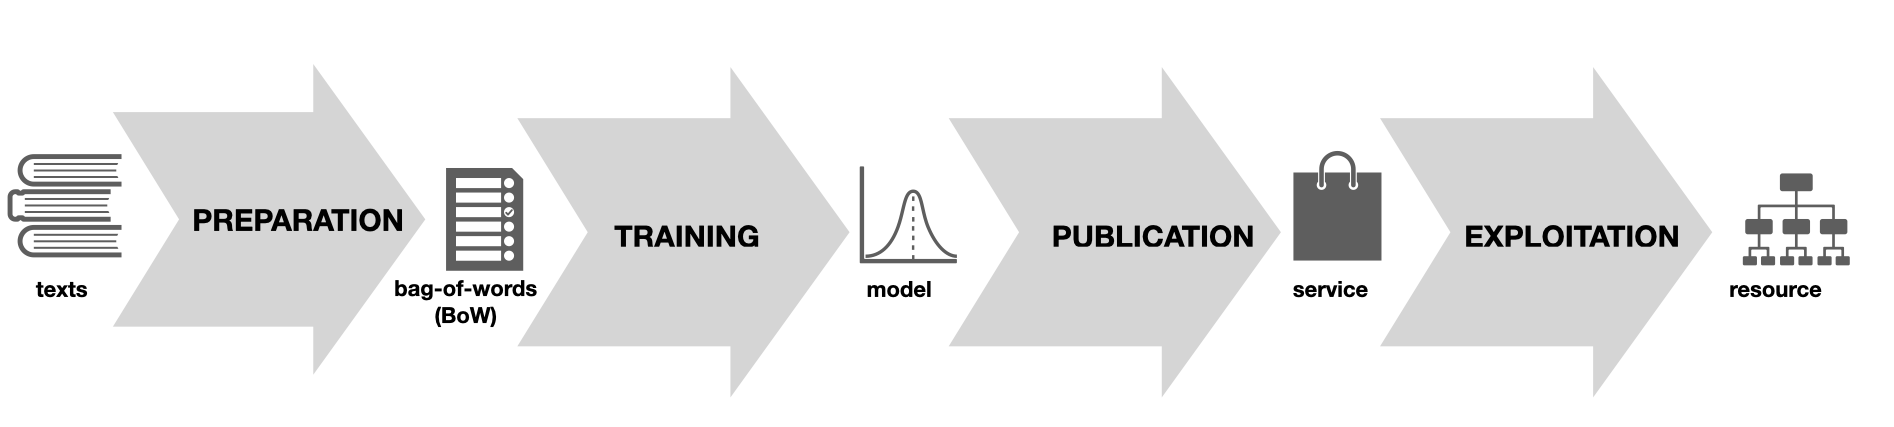
\includegraphics[scale=0.21]{life-cycle.png}
  \caption{Stages in the creation and reuse of topic models. Texts are first processed to retrieve tokens and create bags-of-words (BoW). These structures are used to train a model that identifies word distributions called topics. The model is enabled to make topic inferences in unseen texts. It is published as a web service in an online repository. The service can then be (re)used as web resource, for example to categorize documents.}
  \label{fig:life-cycle}
\end{figure}


\textit{librAIry} is a framework that covers the entire topic model life-cycle by combining learning algorithms with natural language processing methods and software distribution techniques. The main objective is to \textbf{\textit{facilitate the creation of reusable probabilistic topic models by minimizing their technical dependencies}}. Methods and algorithms proposed in this thesis have been implemented and evaluated in this framework, which therefore serves as the technological basis for our research.

Our design requirements, which have guided our development process, can be organized into three categories:
\begin{itemize}
\item \textbf{Corpora representation requirements}, which tackle the modeling of document collections and its metadata. This includes texts and their related annotations.
\item \textbf{Task distribution requirements}, which refer to event management to notify changes in document collections. Coordination of this information is crucial for robust and reproducible results.  
\item \textbf{Process execution requirements}, which capture the operations involved in creating a topic model. The parallel task execution leads to the creation of models.
\end{itemize}

The rest of the section describes how we have adapted existing techniques and standards in \textit{librAIry} to address each of the requirement categories described above. An open, distributed and scalable framework has been developed whose source code is publicly available for reuse\footnote{\url{https://github.com/librairy}} and which is registered in the IP of Comunidad de Madrid with reference M-7342-2016.

\subsection{Corpora Representation for Topic Modeling}
\label{sec:representing-corpora}

Inspired by a Staged Event-Driven Architecture (SEDA) that exchanges messages and handles status changes, our framework is based on \textit{resources} and \textit{actions}. A \textit{resource} can be a \textit{document} that represents raw texts (e.g. a full-text research paper), or a \textit{snippet} of text with a logical part  (e.g. sections, summaries or even phrases grouped by their rhetoric), or a \textit{domain} that contains a dataset of texts (e.g. a conference proceedings) or even an \textit{annotation} made on them (e.g. review comments, named-entities, topics). \textit{Actions} can be executed on resources to change their status (e.g. \textit{create}, \textit{update} or \textit{delete}).

To better illustrate this model, take a sample of the research articles published at the K-CAP 2019 conference\footnote{\url{http://www.k-cap.org/2019}} (see Fig. \ref{fig:librairy-model}). A \textit{document} resource is created for each publication and contains the full text of the article. Each \textit{document} is then associated with several \textit{snippets}, one for each section of the article (e.g. abstract, introduction, conclusions, etc). Finally, a \textit{domain} is created that groups all these \textit{documents} under the same conference. This initial representation can be extended with \textit{annotations}, that can provide more detailed information at different levels (e.g. named-entities, keywords or topics).

% 
\begin{figure}
  \center
  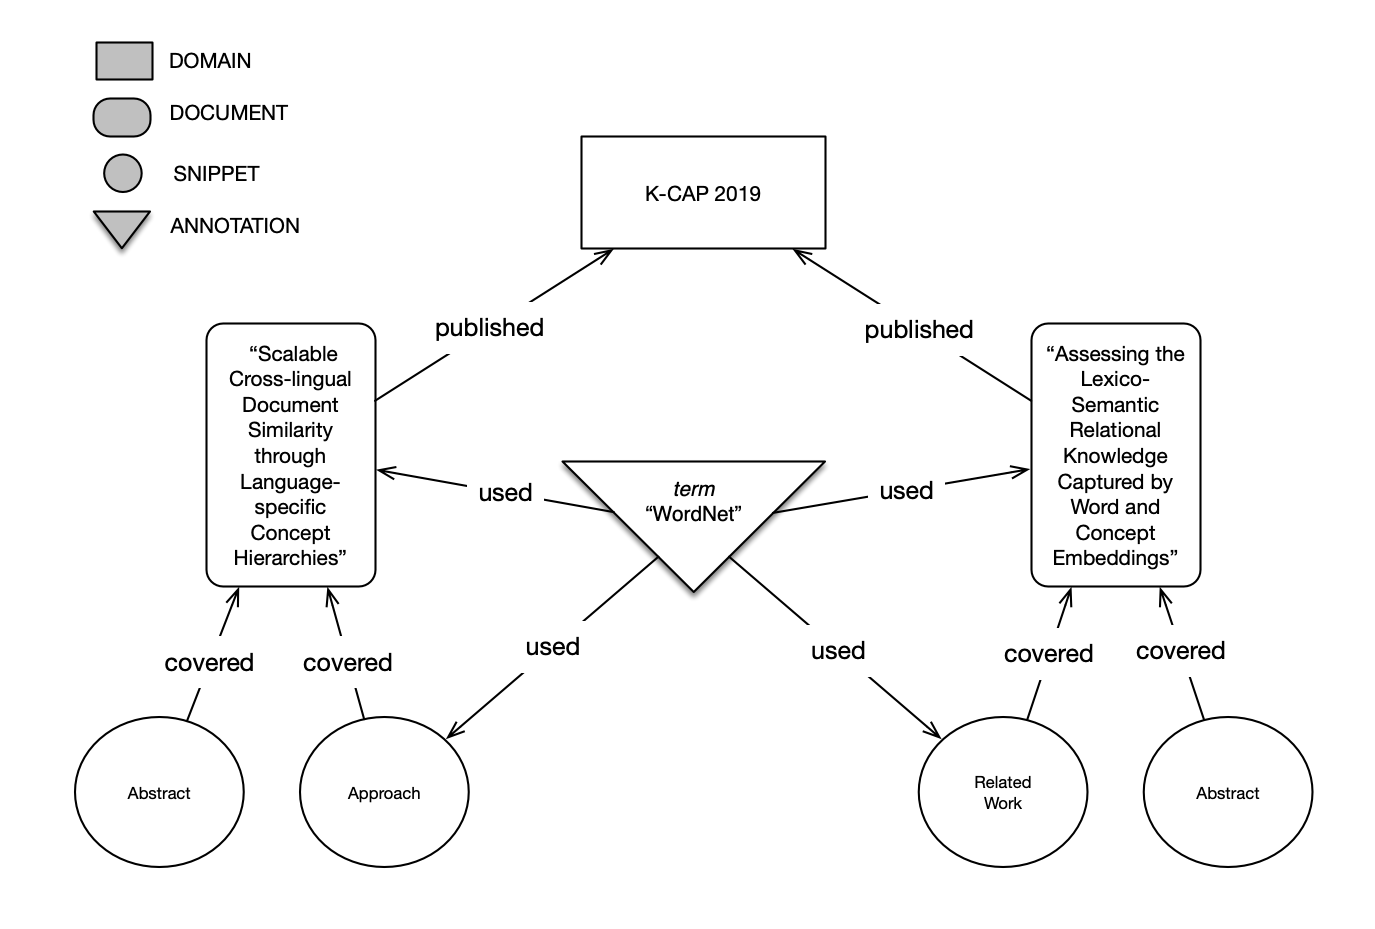
\includegraphics[scale=0.55]{model}
  \caption{Representation of two scientific papers published at the International Conference on Knowledge Capture (K-CAP, 2019) that mention the same entity, \textit{Wordnet}, in different sections.}
  \label{fig:librairy-model}
\end{figure}
% -----------

\textit{Resources} and \textit{actions} are individually addressable and linkable \citep{Turchi2012a} following Linked Data principles \citep{Bizer2009}. Each of them has: (1) a name, (2) a retrievable (or dereferenceable) HTTP URI so that it can be looked up, (3) a descriptive information provided by using standard notation (e.g. JavaScript Object Notation (JSON)) when it is  looked up by URI, and (4) links to other URIs so that other resources can be discovered from it.

More details about each of them is shown below.

\subsubsection{Domain}

A \textit{domain} is an aggregation of \textit{documents}. It is described as a group with parts separately described. Every \textit{document} that is processed belongs, at least, to one \textit{domain} (Fig \ref{fig:librairy-model-domain}).

A \textit{domain} contains the following information: 
\begin{itemize}
\item \textbf{uri}: identifier created from the resource type (i.e \textit{domains}) and a Universally Unique Identifer (UUID) (e.g \textit{domains/88b86fa6-11c8-11eb-adc1-0242ac120002})
\item \textbf{creation-time}: date when resource was created. It follows the ISO-8601\footnote{\url{https://www.iso.org/standard/40874.html}}.
\item \textbf{name}: label associated to the resource.
\item \textbf{description}: additional information about it.
\end{itemize}

\begin{figure}
  \center
  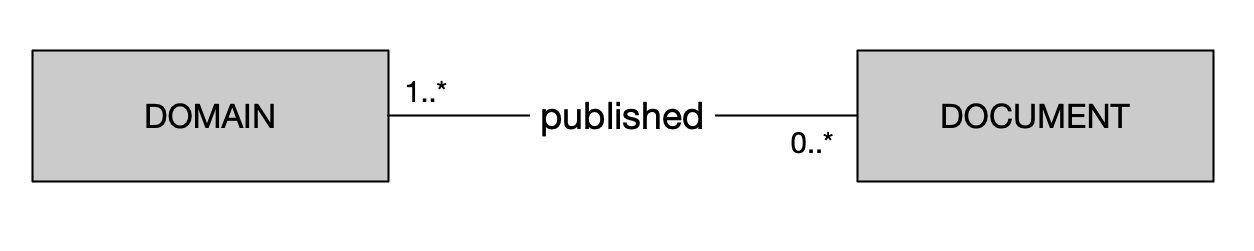
\includegraphics[scale=0.45]{model-domain.png}
  \caption{Relation between \textit{domain} and \textit{document}.}
  \label{fig:librairy-model-domain}
\end{figure}

\subsubsection{Document}

A \textit{document} is a resource consisting primarily of text. Examples include research papers, articles, books or patents. It follows the Open Archives Initiative for Object Reuse and Exchange\footnote{\url{http://www.openarchives.org}} (OAI-ORE) and the Dublin Core Metadata Initiative\footnote{\url{http://dublincore.org}} (DCMI). 

A \textit{document} contains the following information:                                                              

\begin{itemize}
\item \textbf{uri}: identifier created from the resource type (i.e \textit{documents}) and a UUID ( e.g \textit{documents/809af686-11c8-11eb-adc1-0242ac120002})
\item \textbf{creation-time}: date when resource was created. It follows the ISO-8601.
\item \textbf{publishedOn}: date when resource was published. It follows the ISO-8601.
\item \textbf{publishedBy}: an entity responsible for making the document available. It can be a  person, an  organization or a service. It may be different from the entity that conceptually formed the resource (e.g. wrote the document), which is recorded as \textit{authoredBy}. This entity should be identified by a valid Uniform Resource  Identificator (URI) such as WebId\footnote{\url{http://www.w3.org/wiki/WebID}}, orcid\footnote{\url{http://orcid.org}} or internal URI. 
\item \textbf{authoredOn}: the time the \textit{document} was conceptually formed. The author time should be present if different from \textit{publishedOn}. It must be a formatted timestamp following ISO-8601.
\item \textbf{authoredBy}: an entity primarily responsible for making the content of the \textit{document}. It may be a list to indicate multiple authors. Each of them identified by a valid URI such as WebId, orcid or internal URI.
\item \textbf{retrievedFrom}: a URI identifying the repository or source from which the document was derived. This property should be accompanied with \textit{retrievedOn}.
\item \textbf{retrievedOn}: the time the \textit{document} was retrieved on. If this property is present, the \textit{retrievedFrom} must also be present. It must be a formatted timestamp following ISO-8601.
\item \textbf{format}: the physical or digital manifestation of the resource. Typically, it includes the media-type (i.e the IANA code\footnote{\url{http://www.iana.org}}) of the \textit{document}.
\item \textbf{language}: the language(s) in which the document was written. It is defined by RFC-1766\footnote{\url{http://www.ietf.org/rfc/rfc1766.txt}} with a two-letter language code followed, optionally, by a two-letter country code.
\item \textbf{title}: a name given to the \textit{document}. It is a name by which the \textit{document} is formally known.
\item \textbf{description}: it may include but is not limited to an abstract, or a free-text account of the content.
\item \textbf{rights}: information about rights helds in and over the \textit{document}.
\item \textbf{content}: raw text from the \textit{document}.
\end{itemize}

Furthermore, a \textit{document} may contain zero or more \textit{snippets} and a \textit{snippet} may belong to one or more \textit{documents}. Since \textit{librAIry} can also discover relations among \textit{documents}, a \textit{document} may contain zero or more references to other \textit{documents} (Fig. \ref{fig:librairy-model-document}).

\begin{figure}
  \center
  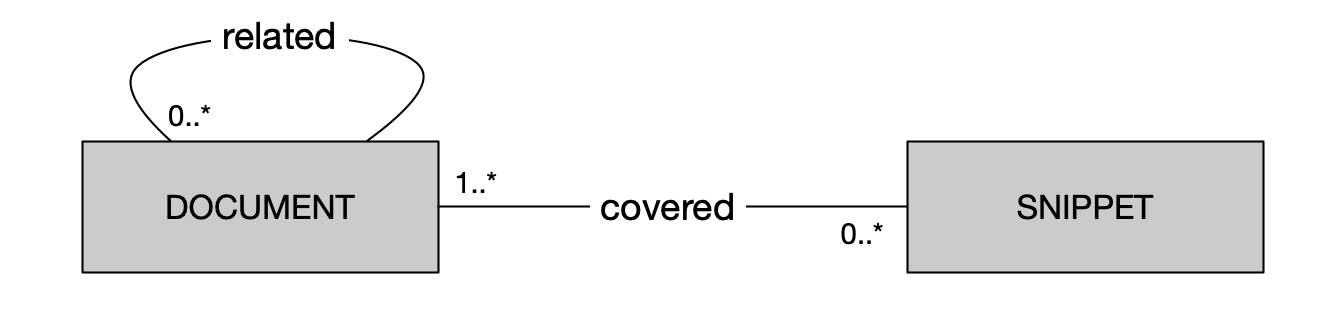
\includegraphics[scale=0.45]{model-document.png}
  \caption{Relation between \textit{document} and \textit{snippet}.}
  \label{fig:librairy-model-document}
\end{figure}

\subsubsection{Snippet}

A \textit{snippet} is a resource that is included either physically or logically in a \textit{document}. In a scientific \textit{document}, for example, it may be the \textit{abstract} section or a logical set of sentences sharing the same rhethorical class (e.g. approach, background, related-work, etc). As seen above (Fig. \ref{fig:librairy-model-document}), a \textit{snippet} can belong to one or more \textit{documents}.

It contains the following information:
\begin{itemize}
\item \textbf{uri}: identifier created from the resource type (i.e \textit{snippets}) and a UUID ( e.g \textit{snippets/7a5a46c8-11c8-11eb-adc1-0242ac120002})
\item \textbf{creation-time}: date when resource was created. It follows the ISO-8601.
\item \textbf{sense}: content-type. It refers to a section or any other criteria under which the following text makes sense (e.g. introduction, summary, notes, etc).
\item \textbf{content}: partial text retrieved from the full-text of a \textit{document}.
\end{itemize}

\subsubsection{Annotation}

\textit{Annotations} are data retrieved from resources that can be used to relate them. They are basically key-value data structures associated to \textit{domains}, \textit{documents} or \textit{snippets}. Examples are entities mentioned in a text, or topics covered in a collection. Any resource can have zero or multiple annotations, which can be shared among several resources (Fig. \ref{fig:librairy-model-annotation})

It contains the following information:
\begin{itemize}
\item \textbf{uri}: identifier created from the resource type (i.e \textit{annotations}) and a UUID ( e.g \textit{annotations/73671e68-11c8-11eb-adc1-0242ac120002})
\item \textbf{creation-time}: date when resource was created. It follows the ISO-8601.
\item \textbf{key}: a category or type associated with the information it contains (e.g. entity, comment, topic, keywords, etc). Recommended best practice is to use a controlled vocabulary.
\item \textbf{value}: a note about the resource in the form of free text.
\end{itemize}

\begin{figure}
  \center
  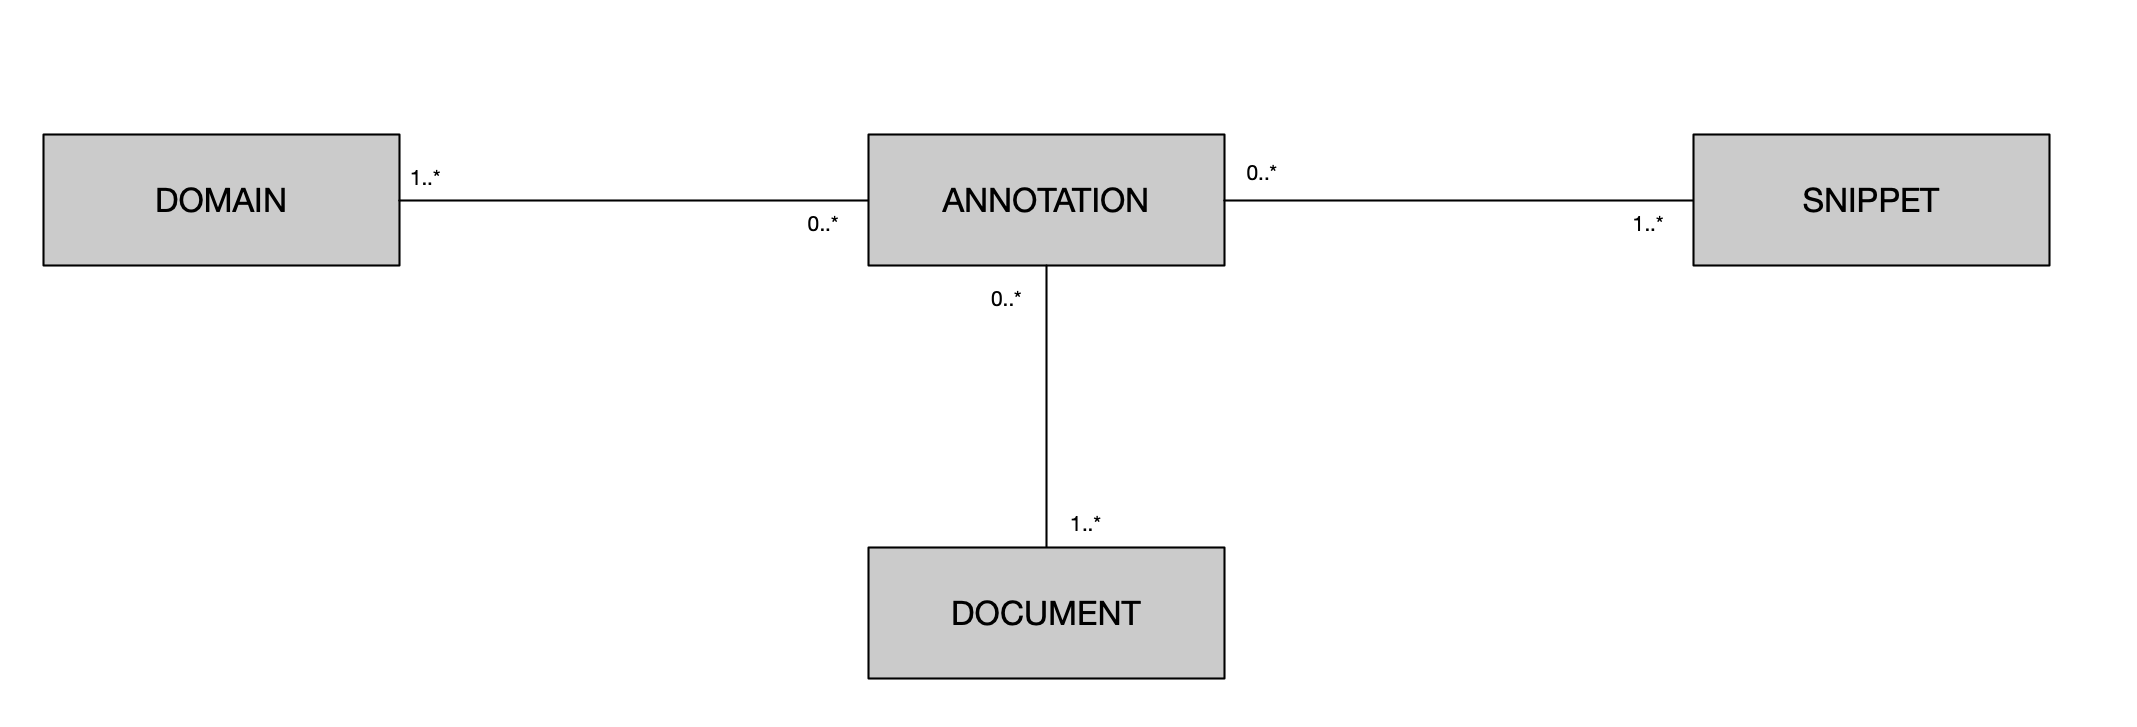
\includegraphics[scale=0.4]{model-annotation.png}
  \caption{Relation between \textit{annotations} and other resources.}
  \label{fig:librairy-model-annotation}
\end{figure}

\subsection{Event-oriented Processing Workflow}

Along with the resources mentioned above, there are two additional elements that provide a crucial behavior to the framework: \textit{modules} and \textit{events}. An \textit{event} is a non-persistent time-based occurrence that describes a new action performed on a resource. \textit{Modules} are responsible for carrying out operations on the resources (e.g. tokenize a \textit{document} or create a topic model from a \textit{domain}). \textit{Events} are broadcasted so that any \textit{module} is aware of the changes made to the resources and  can perform actions on one or more resources in response to a new state reached by a given resource. These actions are paralleled since modules are replicated through distributed environments.

%\begin{figure}
%  \center
%  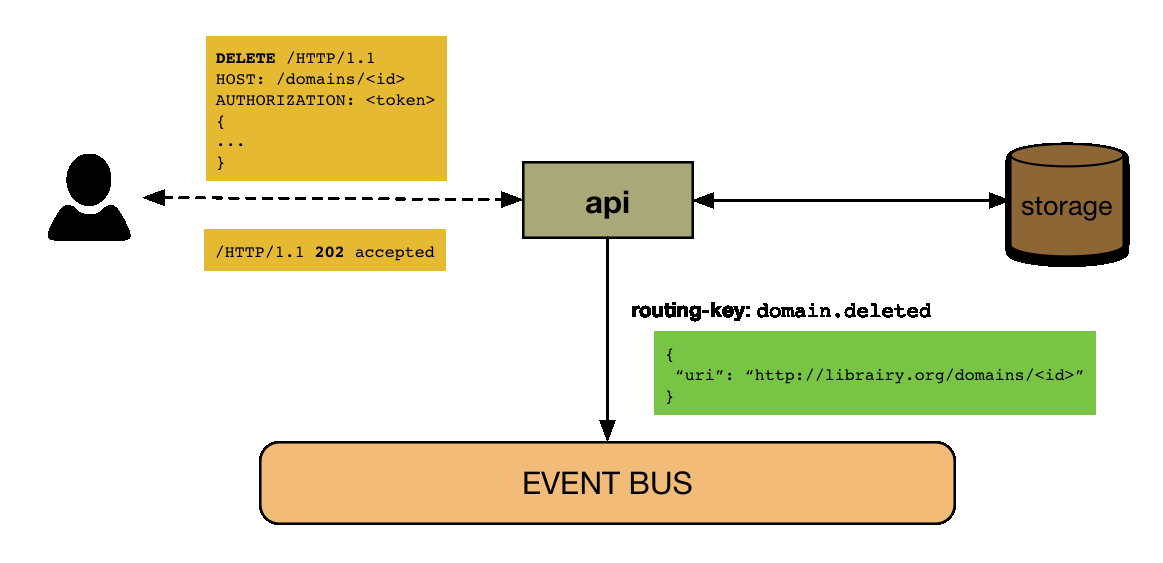
\includegraphics[scale=0.45]{api-domain-deleted}
%  \caption{Domain deleted flow.}
%  \label{fig:librairy-domain-deleted}
%\end{figure}


The framework follows a publisher/subscriber approach where \textit{modules} can publish and read \textit{events} to notify and to be notified about the state of a \textit{resource} (Fig. \ref{fig:librairy-states}). An \textit{event} notifies a performed \textit{action} (i.e. a resource and its new state), and follows the Representational State Transfer (REST) paradigm \citep{Fielding2002}. It contains the resource type and the new state reached by a specific resource ( i.e \textit{created}, \textit{deleted} or \textit{updated}). For example, when a new \textit{domain} is created, an \textit{event} message is published to the channel: $domain.created$. A channel is a space where \textit{events} are published and \textit{modules} can be subscribed to read only some \textit{events}. The actions performed by a module depend on the events to which it is subscribed. Therefore, the workflow of the framework is neither static nor explicitly defined. A distributed dynamic workflow emerges according to the \textit{modules} subscribed to the \textit{event} channels.

From a technical point of view, \textit{librAIry} uses the Advanced Message Queuing Protocol (AMQP) as the messaging standard to avoid any technical dependency to the message broker (i.e the server that sends and receives messages). This protocol defines: \textit{exchanges}, \textit{queues}, \textit{routing-keys} and \textit{binding-keys} to communicate publishers (i.e message senders) and consumers (i.e message readers). \textit{Exchanges} are like message inboxes, and \textit{queues} are subscribed to them by specifying the message types they are interested in with a \textit{binding-key}. A message sent by a publisher to an exchange is routed with a \textit{routing-key} and consumers matching that \textit{routing-key} with their \textit{binding-key} (used to connect the \textit{queue} to that \textit{exchange}), will receive the message. This mechanism allows sending and receiving messages between consumers and producers by means of shared keys (i.e. \textit{routing-keys} and \textit{binding-keys}). A key follows the structure: \textit{resource.status}. Since a wildcard-based definition can be used to set the key, this paradigm allow modules both listening to individual type events (e.g. \textit{domains.created} for new \textit{domains}), or multiple type events (e.g. \textit{\#.created} for all new resources).


\begin{figure}
  \center
  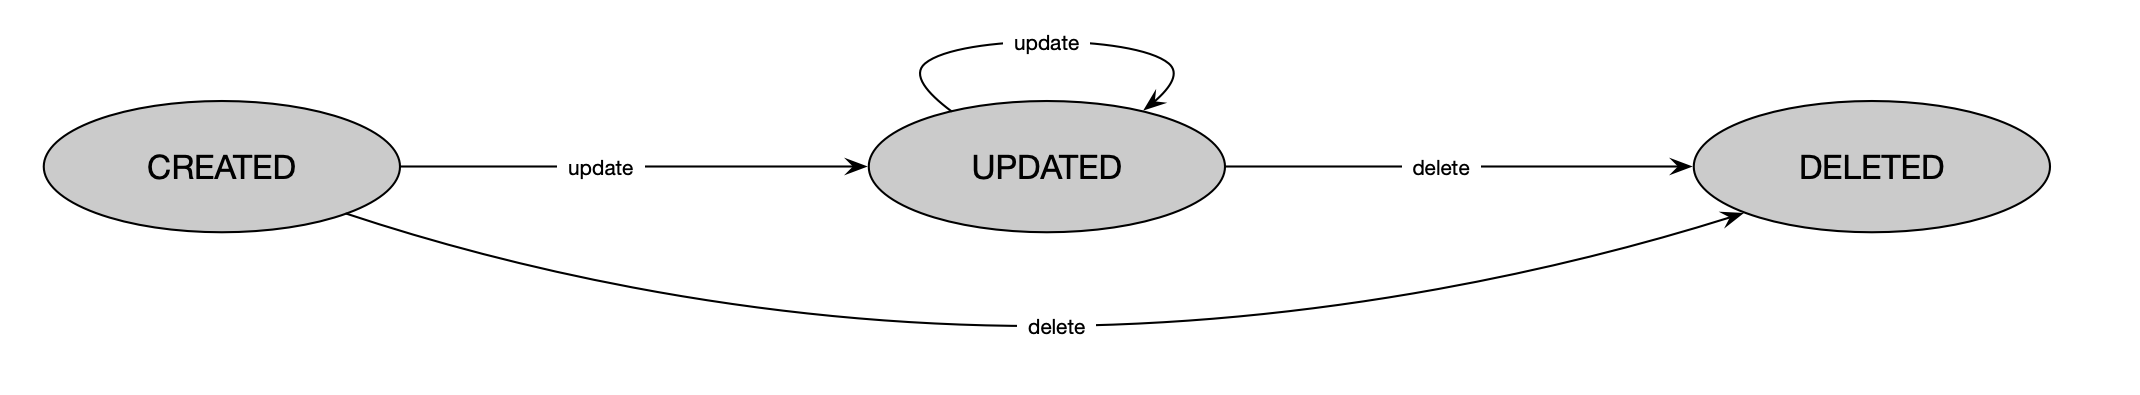
\includegraphics[scale=0.3]{resource-states.png}
  \caption{Resource states.}
  \label{fig:librairy-states}
\end{figure}


\subsection{Module-based Model Training}
\label{sec:librairy-modules}

A microservice-oriented style has been used to define the framework architecture. Using multiple services, the system analyzes texts, creates probabilistic topic models, publishes them as new services and uses them to annotate texts. A service is equivalent to a functionality, and each functionality is materialized by a \textit{module} in the system. A \textit{module} is then a cohesive and independent process \citep{Dragoni2016} with a specific purpose (i.e functionality) based on the \textit{events} to which it responds. These \textit{events} correspond to the routing- and binding- keys attached to the module.

\begin{figure} 
  \center
  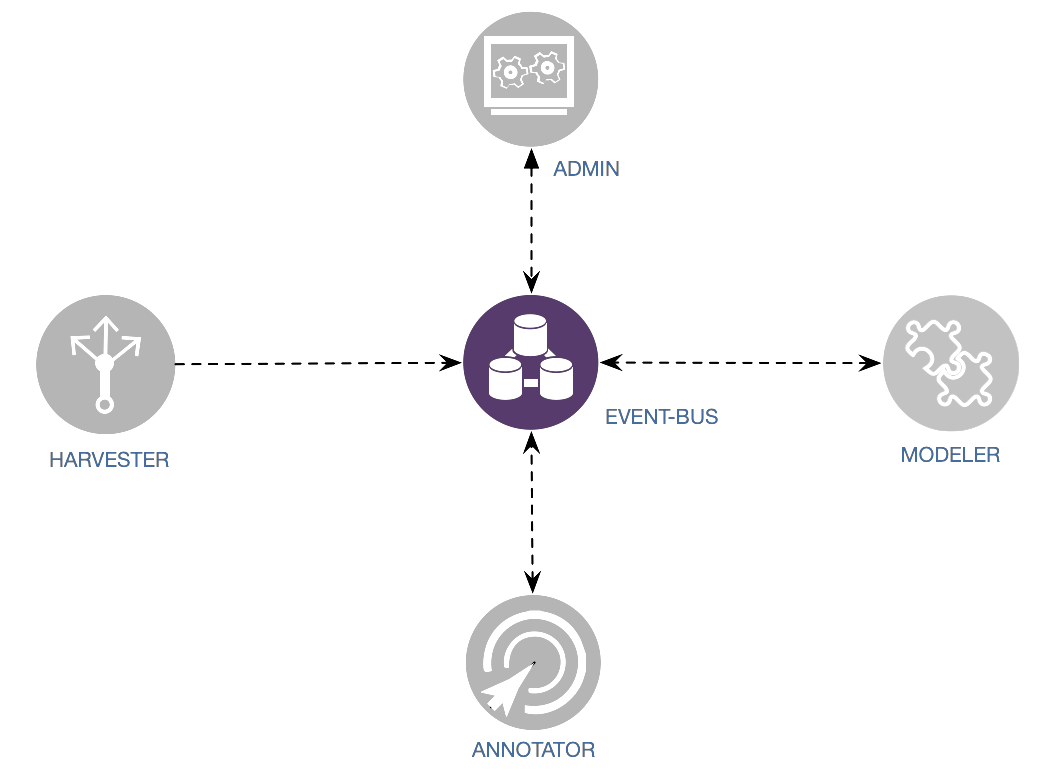
\includegraphics[scale=0.45]{modulesBN}
  \caption{Modules (in gray) publishing or receiving events from the messenger service (in purple).}
  \label{fig:librairy-modules}
\end{figure}


There are four types of \textit{modules} (Fig. \ref{fig:librairy-modules}):
\begin{itemize}
	\item \textbf{Harvester}: creates resources such as \textit{documents}, \textit{snippets} and \textit{domains}, from local or remote repositories with textual files. We have developed harvesters to create scientific resources from Elsevier\footnote{\url{https://github.com/librairy/harvester-elsevier}} or any other digital repository\footnote{\url{https://github.com/librairy/harvester-research}} that follows the Open Archives Initiative Protocol for Metadata Harvesting (OAI-PMH)\footnote{\url{https://github.com/cbadenes/camel-oaipmh}}; as well as more general ones to retrieve public datasets from datos.gob.es\footnote{\url{https://github.com/librairy/harvester-datosGobEs}} or resources located on local folders\footnote{\url{https://github.com/librairy/harvester}}.
    \begin{itemize}
    		\item \textbf{\textit{binding-queue}} (i.e listening for): nothing
		\item \textbf{\textit{routing-key}} (i.e publishing to): \textit{document.created}, \\ \textit{snippet.created}, \textit{domain.(created;updated)}
    \end{itemize}
    \item \textbf{Annotator}: creates \textit{annotations} (e.g named-entities, bag-of-words, topic distributions, etc) in \textit{documents}, \textit{snippets} or \textit{domains}. We have developed an NLP Annotator\footnote{\url{http://librairy.linkeddata.es/nlp}} that creates bag-of-words from a given text by normalizing its content through natural language processing tasks such as named entity recognition, lemmatization or part-of-speech (PoS) tagging. The source code\footnote{\url{https://github.com/librairy/nlp}} is publicly available for reuse. Topic models are also annotators in this framework, as will be seen in section \ref{sec:topic-model-publication}.
    \begin{itemize}
    	\item \textbf{\textit{binding-key}}: \textit{document.(created;updated)}, \textit{snippet.(created;updated)}
	\item \textbf{\textit{routing-key}}: \textit{annotation.(created;deleted)}
    \end{itemize}
    \item \textbf{Modeler}: creates probabilistic topic models for \textit{domains} from the bag-of-word \textit{annotations} of each \textit{document}. We have developed a LDA Modeler\footnote{\url{https://github.com/librairy/modelerTopics-service}} as well as a W2V Modeler\footnote{\url{https://github.com/librairy/modeler-w2v}} (the latter for testing purposes). 
    \begin{itemize}
    	\item \textbf{\textit{binding-key}}: \textit{domain.(created;updated)}, \textit{annotation.created}
	\item \textbf{\textit{routing-key}}: \textit{annotation.(created;deleted)}	
	\end{itemize}
	\item \textbf{Administrator}: performs user-driven tasks such as reading/writing/updating resources or database queries. As with the other modules, the source code\footnote{\url{https://github.com/librairy/api}} is publicly available for reuse. Together with the API, we have also developed a web interface\footnote{\url{https://github.com/librairy/explorer}} to visualize documents, their relationships and the topics associated with each \textit{domain}. 	
    \begin{itemize}
    	\item \textbf{\textit{binding-key}}: \textit{\#.\#}
	\item \textbf{\textit{routing-key}}: \textit{domain.(created;updated;deleted)}, \\ \textit{document.(created;updated;deleted)}, \textit{snippet.(created;updated;deleted)}, \\ \textit{annotation.(created;updated;deleted)}
    \end{itemize}
\end{itemize}


Figure \ref{fig:librairy-sequence} shows a sequence diagram that illustrates how modules work collaboratively to create a topic model from documents added to the framework. Each module provides an Application Program Interface (API) over HTTP, that follows the web standards for the RESTful API development, and a Avro\footnote{\url{https://avro.apache.org}}-based interface over TCP for efficiency reasons. Among them the communication is done over TCP.  

\begin{figure} 
  \center
  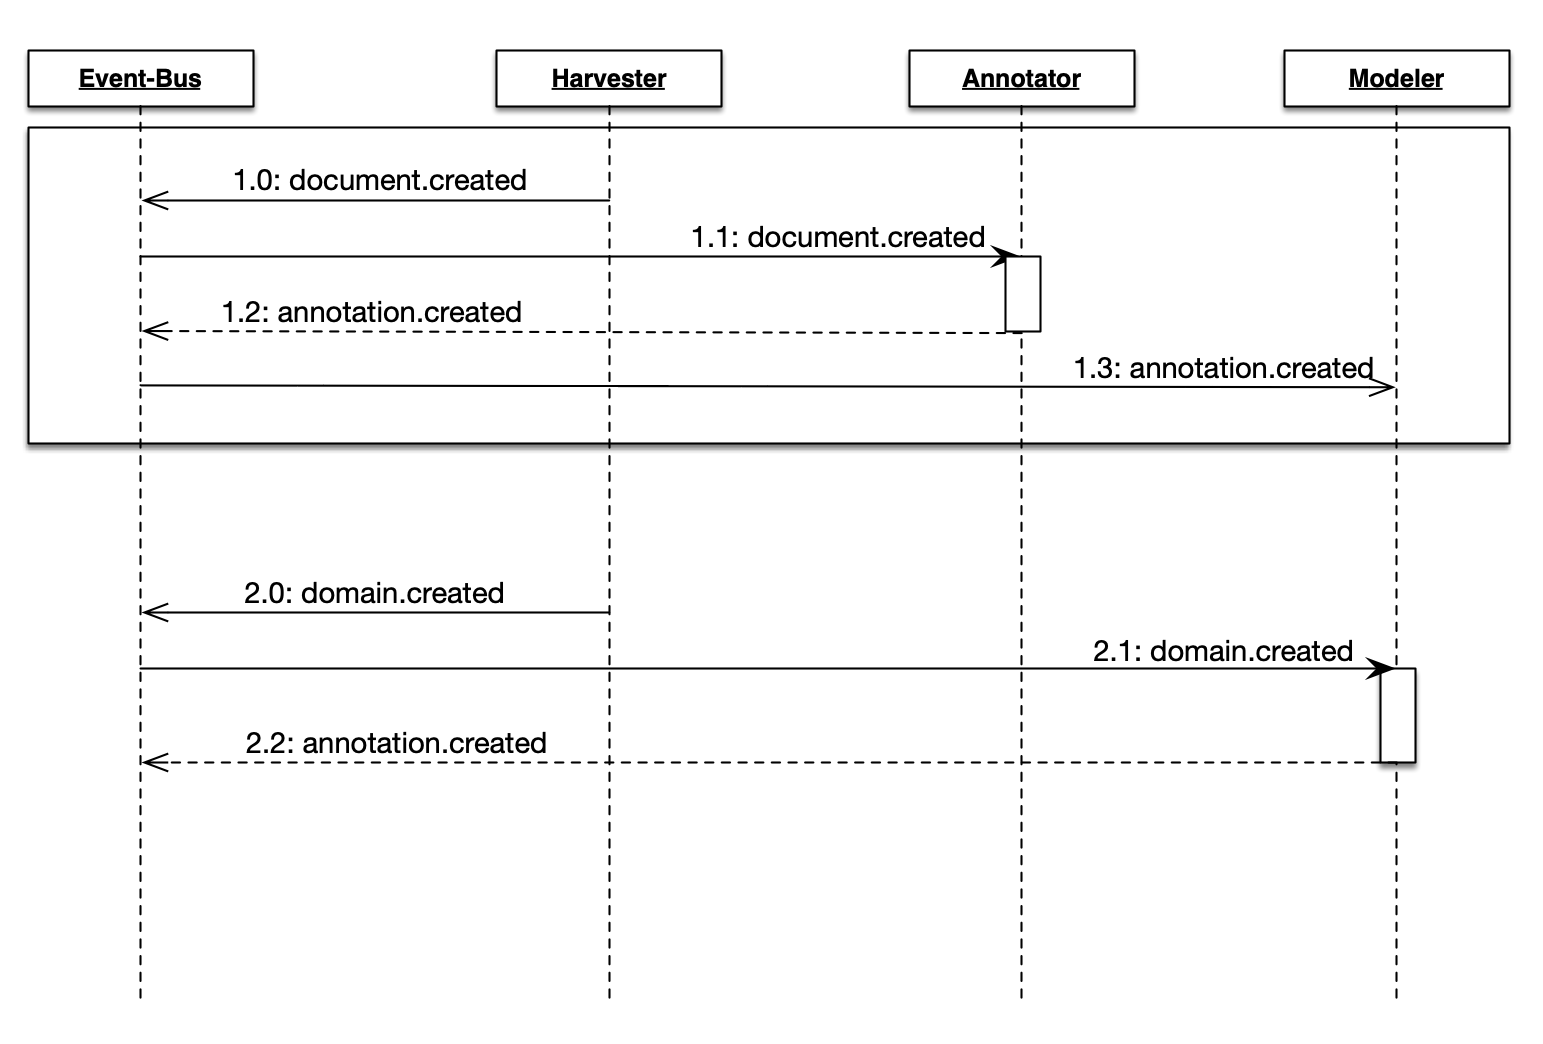
\includegraphics[scale=0.45]{librairy-sequence.png}
  \caption{Sequence of \textit{events} exchanged between modules to create a topic model from the \textit{documents} added to a \textit{domain}.}
  \label{fig:librairy-sequence}
\end{figure}




\section{Topic Modeling Services}
\label{sec:reusable-topic-modeling}

In order to use an existing topic model in our framework, which is micro-services-oriented, the model itself needs to be a service. This approach decouples the resources used to train a probabilistic topic model (e.g. data format or algorithm implementation), from the resources required to  make inferences and thus avoids unexpected incompatibilities. In this way, we simultaneously facilitate the reuse of topic models and also their scalable execution.

\subsection{Topic Model Publication}
\label{sec:topic-model-publication}

We propose distributing topic models as services hosted in online repositories. Models are packaged as OS-level virtualization software that can run reliably applications from one computing environment to another. A model becomes a standalone and executable software package that includes everything needed to use it: code, data, runtime libraries, system tools and settings.

There are several technologies that can virtualize services. Among them, Docker\footnote{\url{https://www.docker.com/}} stands out as a de facto standard due to its wide adoption. It is a platform as a service (PaaS) environment that use operating service-level virtualization to deliver software in packages called \textit{containers}. Containers are isolated from one another and bundle their own software, libraries and configuration files. All containers are run by a single operating system kernel and therefore use fewer resources than virtual machines.

Topic Models in \textit{librAIry} are packaged as Docker \textit{containers} and published in online repositories\footnote{\url{https://hub.docker.com/repositories}} so they can be easily downloaded and run on any machine or software solution. Containers do not only offer virtualization advantages, but also version and license control, since they handle some information that we use to characterize our models:
\begin{itemize}
\item \textbf{repository}: model name (e.g. dbpedia-model).
\item \textbf{author}: model creator (e.g. librAIry)
\item \textbf{version}: model version (e.g. 3.0)
\item \textbf{license}: model license (e.g. Apache 2.0)
\end{itemize}


\subsection{Topic Model Exploitation}
\label{sec:topic-model-exploitation}

Once a topic model has been packaged as a virtual service (i.e. Docker containers), either assembled as a \textit{annotator} in librAIry or as an online service accessible via its HTTP (based on a OpenAPI interface, Fig. \ref{fig:librairy-topic-model-swagger}) or TCP (based on an Avro\footnote{\url{https://github.com/librairy/modeler-service-facade/blob/master/src/main/avro/model.avpr}} interface) API, it should support all tasks that can be performed on a topic model. Taking into account the \textbf{\textit{reproducibility}} of a model, the \textit{conditions under which the model has been created}, in relation to the corpus (i.e. number of documents, vocabulary size, language,.. ), about NLP tasks (i.e stopwords, PoS filtering) and about the model itself (i.e. hyperparameters) should be collected and provided by the service. Taking into account the \textbf{\textit{exploration}} of a model, the \textit{topics and their word distributions} must also be available. The word distribution is usually omitted when publishing topic models providing only the top10 or top5 words per topic. This limits the capacity of the model to be exploited in tasks where that information is required, for example this thesis (as will be seen in chapter 4). And finally, taking into account the topic \textbf{\textit{inference}} in new texts, which is the most extended ability of these models, the service must be able to calculate topic distributions from texts.

\begin{figure} 
  \center
  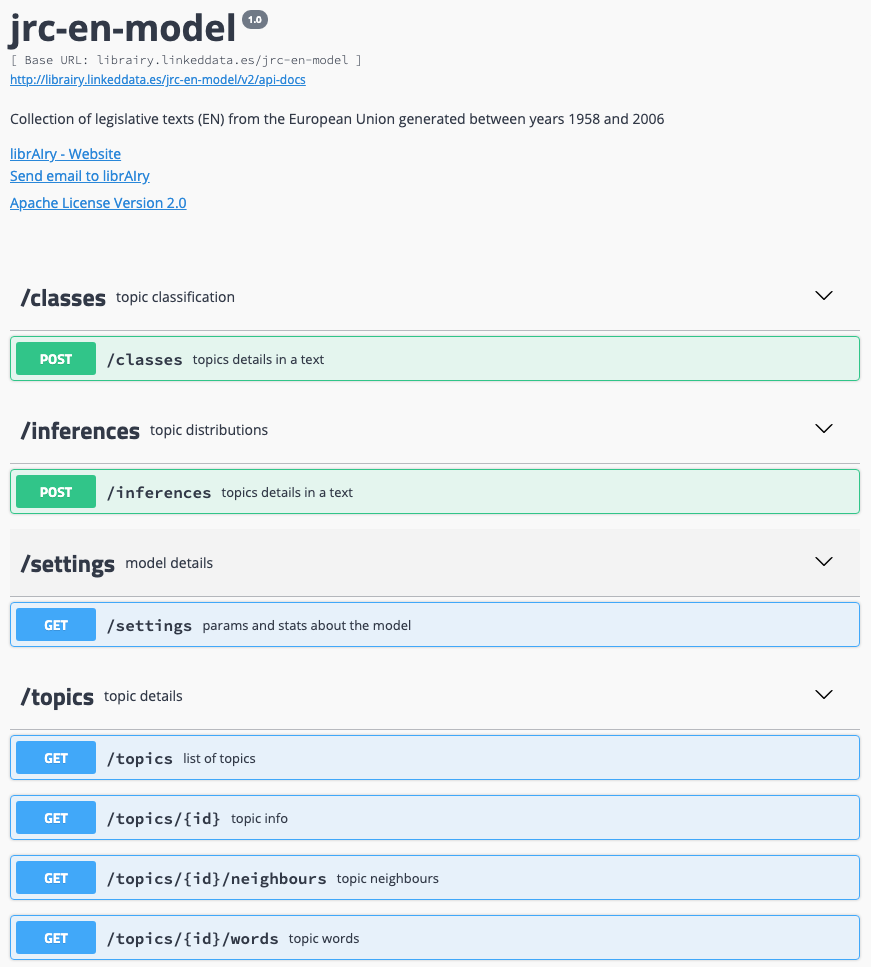
\includegraphics[scale=0.45]{topic-model-swagger.png}
  \caption{OpenAPI-based web interface of a probabilistic topic model service created with \textit{librAIry}.}
  \label{fig:librairy-topic-model-swagger}
\end{figure}


A summary of the tasks, and their purposes, provided by a topic model can be found in Table~\ref{table:tasks}. 

\begin{table}[!htbp]
\centering%
\begin{tabularx}{\linewidth}{bs}
\toprule
\heading{Task} & \heading{Purpose} \\
\midrule
\midrule
T1: Replication & create similar topics\\
\midrule
T2: Exploration & browse topics and words\\
\midrule
T3: Inference & calculate topic distributions\\
\bottomrule
\end{tabularx}
\caption{Potential uses of a topic model.}
\label{table:tasks}
\end{table}

In order to cover these tasks by topic services, the API must offer operations that, individually or partially, allow them to be achieved. A topic model is: \textit{reproducible} (T1) when its hyperparameters and the configuration of the training set are known, \textit{explorable} (T2) when the word distributions of each topic are known, and is \textit{interpretable} (T3) when the presence of each topic can be measured in a text. Table~\ref{table:operations} summarizes the operations offered by a topic model-as-a-service to support the potential uses.

\begin{table}[!htbp]
\small
\centering%
\begin{tabularx}{\linewidth}{bb}
\toprule
\heading{Operations} & \heading{Tasks} \\
\midrule
\midrule
O1: reading of model hyperparameters (i.e alpha, beta, and number of topics) & T1: Replication\\
\midrule
O2: reading of pre-processing tasks (i.e stopwords, normalization, PoS filtering) & T1: Replication\\
\midrule
O3: reading of learning parameters (i.e iterations, seed, likelihood) & T1: Replication \\
\midrule
O4: reading of topics described by word distributions (i.e topic relevance) & T2: Exploration\\
\midrule
O5: reading of words described by topic distributions (i.e word relevance) & T2: Exploration\\
\midrule
O6: calculation of topic distributions in texts (i.e vector of topic distributions) & T3: Inference\\
\bottomrule
\end{tabularx}
\caption{Operations offered by a topic model-as-a-service to cover potential tasks.}
\label{table:operations}
\end{table}

The rest of the section describes how the model implements these operations through service methods. A topic model-as-a-service is online available for review\footnote{\url{http://librairy.linkeddata.es/jrc-en-model}}.

\subsubsection{Reproducibility Tasks}
Through a single request to the model API, a list of parameters is provided to support the O1, O2, and O3 operations. The method is available by both a HTTP-GET request on \textit{\url{/settings}} resource and by a TCP request on \textit{getSettings} method. An online example is available here\footnote{\url{http://librairy.linkeddata.es/jrc-en-model/settings}}. 

A detailed list of the parameters provided by the topic model is shown below:
\begin{itemize}
\item \textbf{algorithm}: method used to train the model (e.g. LDA).
\item \textbf{date}: when the model was created. It follows the ISO-8601.
\item \textbf{params}: configuration of the learning process.
	\begin{itemize}
	\item \textbf{seed}: numerical value to ensure consistent results (e.g. 1066).
	\item \textbf{lowercase}: if true, text is converted to lowercase.
	\item \textbf{topics}: number of topics.
	\item \textbf{language}: language of texts.
	\item \textbf{iterations}: number of sampling iterations.
	\item \textbf{entities}: if true, NER tasks are performed.
	\item \textbf{max-doc-ratio}: maximum word presence per document ratio (e.g. 0.9).
	\item \textbf{min-freq}: minimum word presence per number of document (e.g. 5). 
	\item \textbf{alpha}: prior distribution over topic weights in each document (e.g. 0.1)
	\item \textbf{beta}: prior distribution over word weights in each topic (e.g. 0.01)
	\item \textbf{part-of-speech}: word classes used in the model (e.g. NOUN, VERB, ADJECTIVE)
	\item \textbf{top-words}: number of words used to describe a topic (e.g. 10)
	\item \textbf{stop-words}: list of words removed from the corpus (e.g. quantity, datum) 
	\end{itemize}
\item \textbf{stats}: statistics after the learning process.
	\begin{itemize}
	\item \textbf{loglikelihood}: how much the model fits with the training set.
	\item \textbf{vocabulary}: number of unique words.
	\item \textbf{topic-coherence}: distance between topics from their top words (e.g min, max, mean, mode).
	\item \textbf{topic-distance}: distance between topics from their word distributions (e.g min, max, mean, mode).
	\item \textbf{corpus}: number of documents in the training set. 
	\end{itemize}
\end{itemize}


\subsubsection{Exploration Tasks}
The exploration task, with its respective operations of reading topics (O4) and words (O5), is broken down into four services:

\begin{itemize}
\item \textbf{Topic List}(O4). By means of the HTTP-GET \textit{/topics}\footnote{\url{http://librairy.linkeddata.es/jrc-en-model/topics}} resource and the TCP \textit{getTopics} method, all the topics of the model are listed. Each topic is described with an increasing unique \textit{identifier} (from 0 to the maximum number of topics), a label or \textit{name} in case it has been established, and a \textit{description} with the most relevant words (based on their density distributions). 
\item \textbf{Topic Detail}(O4). By means of the HTTP-GET \textit{\url{/topics/_id_}}\footnote{\url{http://librairy.linkeddata.es/jrc-en-model/topics/0}} resource and the TCP \textit{getTopic} method, a topic identified by \textit{id} is described by providing its \textit{identifier}, \textit{name}, \textit{description} and \textit{entropy} (i.e how different is with respect the other topics).
\item \textbf{Topic Words}(O5). By means of the HTTP-GET \textit{\url{/topics/_id_/words}}\footnote{\url{http://librairy.linkeddata.es/jrc-en-model/topics/0/words}} resource and the TCP \textit{getTopicWords} method, a list of word distributions for the topic identified by \textit{id} is provided. Every word has its weight (i.e relevance score) with respect to the topic.
\item \textbf{Topic Neighbours}(O4). By means of the HTTP-GET \textit{\url{/topics/_id_/neighbours}}\footnote{\url{http://librairy.linkeddata.es/jrc-en-model/topics/0/neighbours}} resource and the TCP \textit{getTopicNeighbours} method, a list of topics related to the topic identified by \textit{id} is provided. The distance between topics is measured from their word distributions.  
\end{itemize}

\subsubsection{Inference Tasks}

A single request with the text to be analyzed returns a list with the presence of each topic (O5) in that text. The method is available by both a HTTP-POST request to \textit{\url{/inferences}} or a TCP request to the  \textit{createInference} method, with a JSON message containing the text  to be analyzed.

% existentes herramientas de análisis de textos: escalabilidad vertical

% en que consiste los modelos probabilísticos de tópicos para necesitar tareas de NLP


%In natural language processing, the term topic means a set of words. These are the words that come to mind when thinking of this topic. For example music could associate the words sound, instrument and composition. Without going more deep now, a topic model automatically discovers the words that are most likely to describe the topics present in a document collection. A trained model may then be used to infer which of these topics occur in new documents and can also pick out which portions of a document cover which topics.

%The learning process in a topic model first requires creating bag-of-words (BoW) from texts. A BoW contains the frequencies of each word in a text. The model uses these representations to discover the word distributions that best define the topics to fit their presences in the documents, assuming that a document can covers several topics. Take the following text: "Apple has just released in its Apple Store a video celebrating International Women's Day, about the lives of several relevant women, especially the most influential young woman in recent years.". A basic approach would transform that text into a BoW that considers whitespaces and punctuation marks as word separators (e.g. 'Apple'(2), 'has'(1), 'just'(1), etc). But this approach makes several mistakes. 'Apple' does not appear twice, but only once, as 'Apple Store' is different to 'Apple'. Some natural language processing tasks are needed to make these assessments. Using Named Entity Recognition (NER) techniques, for example,  'Apple', 'Apple Store' and 'International Women's Day' are different words in a BoW. Sometimes a normalization is applied to group plural and singular nouns. Using stemming techniques and Part-of-Speech (PoS) tagging, 'women' and 'woman' are transformed into a same word, 'woman', with a frequency equals to the sum of their frequencies, in this case 2. This is just a very simple illustration of how texts need to be processed to train probabilistic topic models. 

%While most topic model tools already include such functionality, they have not taken into account integration and scalability issues in their development. It is difficult, and sometimes impossible, to incorporate external resources into the workflow to perform some of these tasks (e.g. NER, PoS Tagging, etc) due to incompatibility problems. They can appear at the data level with different annotation categories (e.g. AnCora and CoNLL-U tagsets for PoS tagging), or at the execution level with different technological stacks (e.g. Java and Python). Furthermore, they are mainly focused on vertical scalability (better processing machines), instead of horizontal scalability (more processing machines). There are tools that have recently addressed, although only partially, some of these incompatibilities\footnote{\url{https://www.openml.org}}. But, as far as we know, these approaches keep forgetting the horizontal scalability in their designs. Only with high-performance machines can huge document collections be processed, instead of combining some lower-performance machines.

%We propose a distributed framework where multiple and heterogeneous text mining tools can collaboratively work. A shared workflow emerges to combine external tools (e.g. java-based and python-based tools to create topic models and NLP tasks), that may be located on different machines and even replicated at different scales. This raises both technical and functional challenges to coordinate distributed executions. From the technical point of view, isolated environments and communication mechanisms are required so dissimilar tools can be executed with maximum guarantees. From the functional point of view, all executions must be coordinated to reach a final result as aggregation of partial results derived from each execution.

 


%\subsubsection{Storage}

%Multiple types of data can be handled in this ecosystem. Inspired in the Data Access Object (DAO) pattern, we have created a Unified Data Manager (UDM) providing access to any type of data used in the system.  Three types of databases have been considered:
%\begin{itemize}
	%\item \textbf{column-oriented database}: Focused on unique identified and/or \textit{structured data}. This storage allow %us searching key elements across resources. 
	%\item \textbf{document-oriented database}: Focused on indexing raw text. This storage allow us to execute advanced search %operations over all the information gathered about a textual resource. 
    %\item \textbf{graph database}: Focused on relations. This storage allow us exploring resources through the relationships %between them.
%\end{itemize}


\section{Summary}

In Section \ref{sec:topic-model-framework} we have described \textit{librAIry}, the framework to cover the entire topic model life-cycle in a scalable way. Algorithms and tools coming from different technologies work collaboratively to process and analyze huge collections of textual resources creating and using probabilistic topic models. 

We tested and validated \textit{librAIry} by using the framework in some real world scenarios such as DrInventor\footnote{\url{http://drinventor.eu}}, where thousands of scientific publications were processed, TheyBuyForYou\footnote{\url{https://theybuyforyou.eu}}, where hundreds of thousands of public procurement texts were analyzed, or 
CorpusViewer\footnote{\url{https://www.plantl.gob.es/tecnologias-lenguaje/actividades/plataformas/Paginas/corpus-viewer.aspx}}, where millions of patents were automatically organized. Thus, \textit{librAIry} has proven to be a valid and scalable text processing framework and addresses the first technical objective of this thesis ( T01, \textit{create a scalable platform for  topic modeling}).

\textit{librAIry} has been designed to represent corpora by organizing the data in three levels of detail: \textit{snippets} to reflect parts or pieces of texts, \textit{documents} to represent full texts, and \textit{domains} to group documents. Transversally there are \textit{annotations}, which allow providing more details to any of them. Figure \ref{fig:librairy-model} shows how two scientific articles published in the same conference and that mention a same resource in their papers can be represented. On this representation model based on SEDA architectures, actions over resources and status change notification events are introduced, which enable to distribute the processing of resources. Figure \ref{fig:librairy-modules} shows the four modules involved in processing the resources. \textit{Harvester} modules create new \textit{documents}, \textit{snippets} and \textit{domains}. \textit{Annotator} modules react to each new resource and introduce \textit{annotations}. \textit{Modeler} modules create new topic models for each new \textit{domain}. And \textit{Admin} modules perform administrative tasks and allow users to read the data. As shown in figure \ref{fig:librairy-sequence}, modules coordinate their actions by reacting to the notifications. The actions are then executed in parallel through a distributed workflow and the first research objective of this thesis is addressed (RO1, \textit{define a distributed text-processing model for creating large probabilistic topic models}).

In Section \ref{sec:reusable-topic-modeling} we propose the publication of topic models as web services that can be used from external solutions or integrated into the \textit{librAIry} framework. Regardless of their API, since they work both over HTTP and over TCP, there are three types of tasks that guide the definition of the service: \textit{reproducibility}, \textit{exploration}, and \textit{inference}. Tables~\ref{table:tasks} and \ref{table:operations} detail the operations  supported by the service to cover these tasks. The definition of a topic model-as-a-service covers the second research objective of this thesis (R02, \textit{define a template to package probabilistic topic models as web services}).
 
And finally, in order to facilitate the reuse of the topic models published as web services, section \ref{sec:topic-model-publication} presents an online repository based on virtual services. This covers the second technical objective of the thesis (T02, \textit{create a repository of topic-based web services}). 
 
%A new model definition based on the previously mentioned principle of maximizing information re-usability and minimize irrelevant data has been studied to create a fine-grained resource design. New domains, in the sense of particular vocabularies or specific textual formats, have been also analyzed to be included into the system via specific harvesters or more precise annotators. Moreover, a template-based mechanism oriented to facilitate the integration of new tools and techniques into the system has been built to make easier to develop new modules as well as increasing the available modules in public repositories.

%Our approach to create and inference probabilistic topics is \textbf{scalable} enough to work properly in both situations. This chapter presents a framework for processing topic models in document collections ranging from only a few texts, to large scale corpora. Methods and algorithms proposed in this thesis have been implemented and evaluated in this environment, which therefore serves as the technological basis for our research. The motivation is twofold, on the one hand to create a scalable system to analyze documents and discover topics, and on the other hand to create reusable topic models that can be easily integrated into that system.
